\documentclass[tikz,margin=.1in]{standalone}
\usepackage{pgfplots,lmodern}
\pgfplotsset{compat=newest}

\begin{document}
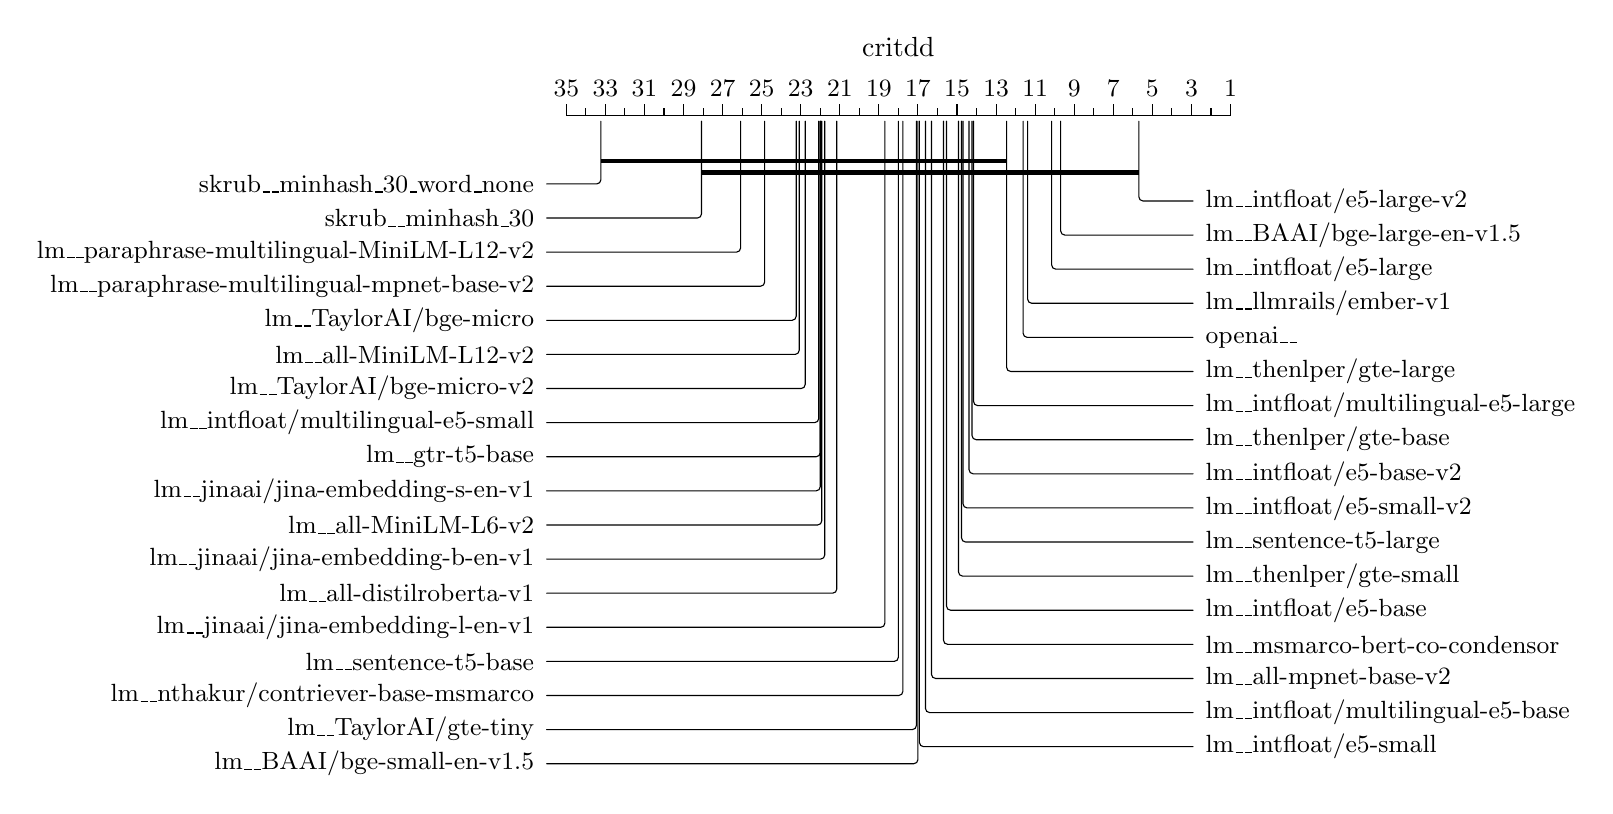
\begin{tikzpicture}[
  treatment line/.style={rounded corners=1.5pt, line cap=round, shorten >=1pt},
  treatment label/.style={font=\small},
  group line/.style={ultra thick},
]

\begin{axis}[
  clip={false},
  axis x line={center},
  axis y line={none},
  axis line style={-},
  xmin={1},
  ymax={0},
  scale only axis={true},
  width={\axisdefaultwidth},
  ticklabel style={anchor=south, yshift=1.3*\pgfkeysvalueof{/pgfplots/major tick length}, font=\small},
  every tick/.style={draw=black},
  major tick style={yshift=.5*\pgfkeysvalueof{/pgfplots/major tick length}},
  minor tick style={yshift=.5*\pgfkeysvalueof{/pgfplots/minor tick length}},
  title style={yshift=\baselineskip},
  xmax={35},
  ymin={-18.5},
  height={19\baselineskip},
  xtick={1,3,5,7,9,11,13,15,17,19,21,23,25,27,29,31,33,35},
  minor x tick num={1},
  x dir={reverse},
  title={critdd},
]

\draw[treatment line] ([yshift=-2pt] axis cs:5.6923076923076925, 0) |- (axis cs:2.775641025641026, -2.5)
  node[treatment label, anchor=west] {lm\_\_intfloat/e5-large-v2};
\draw[treatment line] ([yshift=-2pt] axis cs:9.692307692307692, 0) |- (axis cs:2.775641025641026, -3.5)
  node[treatment label, anchor=west] {lm\_\_BAAI/bge-large-en-v1.5};
\draw[treatment line] ([yshift=-2pt] axis cs:10.153846153846153, 0) |- (axis cs:2.775641025641026, -4.5)
  node[treatment label, anchor=west] {lm\_\_intfloat/e5-large};
\draw[treatment line] ([yshift=-2pt] axis cs:11.384615384615385, 0) |- (axis cs:2.775641025641026, -5.5)
  node[treatment label, anchor=west] {lm\_\_llmrails/ember-v1};
\draw[treatment line] ([yshift=-2pt] axis cs:11.615384615384615, 0) |- (axis cs:2.775641025641026, -6.5)
  node[treatment label, anchor=west] {openai\_\_};
\draw[treatment line] ([yshift=-2pt] axis cs:12.461538461538462, 0) |- (axis cs:2.775641025641026, -7.5)
  node[treatment label, anchor=west] {lm\_\_thenlper/gte-large};
\draw[treatment line] ([yshift=-2pt] axis cs:14.153846153846153, 0) |- (axis cs:2.775641025641026, -8.5)
  node[treatment label, anchor=west] {lm\_\_intfloat/multilingual-e5-large};
\draw[treatment line] ([yshift=-2pt] axis cs:14.23076923076923, 0) |- (axis cs:2.775641025641026, -9.5)
  node[treatment label, anchor=west] {lm\_\_thenlper/gte-base};
\draw[treatment line] ([yshift=-2pt] axis cs:14.384615384615385, 0) |- (axis cs:2.775641025641026, -10.5)
  node[treatment label, anchor=west] {lm\_\_intfloat/e5-base-v2};
\draw[treatment line] ([yshift=-2pt] axis cs:14.692307692307692, 0) |- (axis cs:2.775641025641026, -11.5)
  node[treatment label, anchor=west] {lm\_\_intfloat/e5-small-v2};
\draw[treatment line] ([yshift=-2pt] axis cs:14.76923076923077, 0) |- (axis cs:2.775641025641026, -12.5)
  node[treatment label, anchor=west] {lm\_\_sentence-t5-large};
\draw[treatment line] ([yshift=-2pt] axis cs:14.923076923076923, 0) |- (axis cs:2.775641025641026, -13.5)
  node[treatment label, anchor=west] {lm\_\_thenlper/gte-small};
\draw[treatment line] ([yshift=-2pt] axis cs:15.538461538461538, 0) |- (axis cs:2.775641025641026, -14.5)
  node[treatment label, anchor=west] {lm\_\_intfloat/e5-base};
\draw[treatment line] ([yshift=-2pt] axis cs:15.692307692307692, 0) |- (axis cs:2.775641025641026, -15.5)
  node[treatment label, anchor=west] {lm\_\_msmarco-bert-co-condensor};
\draw[treatment line] ([yshift=-2pt] axis cs:16.307692307692307, 0) |- (axis cs:2.775641025641026, -16.5)
  node[treatment label, anchor=west] {lm\_\_all-mpnet-base-v2};
\draw[treatment line] ([yshift=-2pt] axis cs:16.615384615384617, 0) |- (axis cs:2.775641025641026, -17.5)
  node[treatment label, anchor=west] {lm\_\_intfloat/multilingual-e5-base};
\draw[treatment line] ([yshift=-2pt] axis cs:16.923076923076923, 0) |- (axis cs:2.775641025641026, -18.5)
  node[treatment label, anchor=west] {lm\_\_intfloat/e5-small};
\draw[treatment line] ([yshift=-2pt] axis cs:17.0, 0) |- (axis cs:36.1474358974359, -19.0)
  node[treatment label, anchor=east] {lm\_\_BAAI/bge-small-en-v1.5};
\draw[treatment line] ([yshift=-2pt] axis cs:17.076923076923077, 0) |- (axis cs:36.1474358974359, -18.0)
  node[treatment label, anchor=east] {lm\_\_TaylorAI/gte-tiny};
\draw[treatment line] ([yshift=-2pt] axis cs:17.76923076923077, 0) |- (axis cs:36.1474358974359, -17.0)
  node[treatment label, anchor=east] {lm\_\_nthakur/contriever-base-msmarco};
\draw[treatment line] ([yshift=-2pt] axis cs:18.0, 0) |- (axis cs:36.1474358974359, -16.0)
  node[treatment label, anchor=east] {lm\_\_sentence-t5-base};
\draw[treatment line] ([yshift=-2pt] axis cs:18.692307692307693, 0) |- (axis cs:36.1474358974359, -15.0)
  node[treatment label, anchor=east] {lm\_\_jinaai/jina-embedding-l-en-v1};
\draw[treatment line] ([yshift=-2pt] axis cs:21.153846153846153, 0) |- (axis cs:36.1474358974359, -14.0)
  node[treatment label, anchor=east] {lm\_\_all-distilroberta-v1};
\draw[treatment line] ([yshift=-2pt] axis cs:21.76923076923077, 0) |- (axis cs:36.1474358974359, -13.0)
  node[treatment label, anchor=east] {lm\_\_jinaai/jina-embedding-b-en-v1};
\draw[treatment line] ([yshift=-2pt] axis cs:21.923076923076923, 0) |- (axis cs:36.1474358974359, -12.0)
  node[treatment label, anchor=east] {lm\_\_all-MiniLM-L6-v2};
\draw[treatment line] ([yshift=-2pt] axis cs:22.0, 0) |- (axis cs:36.1474358974359, -11.0)
  node[treatment label, anchor=east] {lm\_\_jinaai/jina-embedding-s-en-v1};
\draw[treatment line] ([yshift=-2pt] axis cs:22.0, 0) |- (axis cs:36.1474358974359, -10.0)
  node[treatment label, anchor=east] {lm\_\_gtr-t5-base};
\draw[treatment line] ([yshift=-2pt] axis cs:22.076923076923077, 0) |- (axis cs:36.1474358974359, -9.0)
  node[treatment label, anchor=east] {lm\_\_intfloat/multilingual-e5-small};
\draw[treatment line] ([yshift=-2pt] axis cs:22.76923076923077, 0) |- (axis cs:36.1474358974359, -8.0)
  node[treatment label, anchor=east] {lm\_\_TaylorAI/bge-micro-v2};
\draw[treatment line] ([yshift=-2pt] axis cs:23.076923076923077, 0) |- (axis cs:36.1474358974359, -7.0)
  node[treatment label, anchor=east] {lm\_\_all-MiniLM-L12-v2};
\draw[treatment line] ([yshift=-2pt] axis cs:23.23076923076923, 0) |- (axis cs:36.1474358974359, -6.0)
  node[treatment label, anchor=east] {lm\_\_TaylorAI/bge-micro};
\draw[treatment line] ([yshift=-2pt] axis cs:24.846153846153847, 0) |- (axis cs:36.1474358974359, -5.0)
  node[treatment label, anchor=east] {lm\_\_paraphrase-multilingual-mpnet-base-v2};
\draw[treatment line] ([yshift=-2pt] axis cs:26.076923076923077, 0) |- (axis cs:36.1474358974359, -4.0)
  node[treatment label, anchor=east] {lm\_\_paraphrase-multilingual-MiniLM-L12-v2};
\draw[treatment line] ([yshift=-2pt] axis cs:28.076923076923077, 0) |- (axis cs:36.1474358974359, -3.0)
  node[treatment label, anchor=east] {skrub\_\_minhash\_30};
\draw[treatment line] ([yshift=-2pt] axis cs:33.23076923076923, 0) |- (axis cs:36.1474358974359, -2.0)
  node[treatment label, anchor=east] {skrub\_\_minhash\_30\_word\_none};
\draw[group line] (axis cs:5.6923076923076925, -1.6666666666666667) -- (axis cs:28.076923076923077, -1.6666666666666667);
\draw[group line] (axis cs:12.461538461538462, -1.3333333333333333) -- (axis cs:33.23076923076923, -1.3333333333333333);

\end{axis}
\end{tikzpicture}
\end{document}
